\documentclass[12pt, a4paper, oneside]{article}
\usepackage{amsmath, amsthm, amssymb, appendix, bm, graphicx, hyperref, mathrsfs, makecell}
\usepackage{bbm, stfloats, subfigure, pythonhighlight, CJK, algorithm, algorithmicx, algpseudocode}
\usepackage{geometry}
\usepackage{float}
\geometry{a4paper,left=2.5cm,right=2.5cm,top=3cm,bottom=3cm}

%\title{\textbf{Title}}
%\author{Min}
%\date{\today}
\linespread{1.6}
\definecolor{lightBlue}{rgb}{0.274,0.41,0.879}
\definecolor{darckGreen}{rgb}{0.1797,0.543,0.3398}
%{\color{lightBlue}Text Here}
\newtheorem{theorem}{Theorem}[section]
\newtheorem{definition}[theorem]{Definition}
\newtheorem{lemma}[theorem]{Lemma}
\newtheorem{corollary}[theorem]{Corollary}
\newtheorem{example}[theorem]{Example}
\newtheorem{proposition}[theorem]{Proposition}
\newtheorem{remark}[theorem]{Remark}
\renewcommand{\abstractname}{\Large\textbf{Abstract}}
\floatname{algorithm}{Algorithm}
\renewcommand{\algorithmicrequire}{\textbf{Input:}}
\renewcommand{\algorithmicensure}{\textbf{Output:}}

\begin{document}
%\maketitle

\setcounter{page}{1}
\pagenumbering{arabic}

\section[Section title sans citation]{Prototypical Concept Learning}

\subsection{Basic set up}
\begin{itemize}
    \item \textbf{The hypothesis space:} consider our training instances to be $S \times \{0, 1\}$ – including both positive and negative
    examples of the target concept – such that training instances are generated by a fixed unknown probability distribution $D$ over $X$ ($D$ is unknown over $X \times Y$).
    \item \textbf{A (data, label) tuple as training samples}: 
    \\$S = [(x_1, f(x_1)), (x_2, f(x_2)),\cdots,(x_n, f(x_n))]$, where each is drawn independently from $D$.
    \item \textbf{One global assumption:} both training and testing instances are drawn from the same distribution $D$.
    \item \textbf{Goal:} determine a hypothesis $h \in H$ that estimates $f$, evaluated by its performance on subsequent instances $x \in X$ drawn according to $D$.
\end{itemize}

\subsection{Motivation}
\begin{itemize}
    \item How much do the results really tell you?
    \item Can we be certain about how the learning algorithm generalizes? 
    \item We would have to see all the examples. (Not practical)
\end{itemize}
\textbf{Insight:} Introduce probabilities to measure degree of certainty and 
correctness. (Valiant 1984)

\subsection{Proposal of ‘Error’}
Consider the error as the probability of an example having different labels according to the hypothesis and the target function, given by
\begin{equation*}
    Error_D = Pr_{x \in D}(f(x) \notin h(x)).
\end{equation*}

\begin{example}[Intuitive example]
    showing the space predicted by target function $f$ and hypothesis function $h$, where points inside the circle are positive, points outside are negative, and the functions are given by
    \begin{gather*}
        h = x_1 \vee x_2 \vee x_3 \vee x_4 \vee x_5, \quad f = x_2 \vee x_3 \vee x_4 \vee x_5
    \end{gather*}
\end{example}
\begin{figure*}[h]
    \centering % 使图片居中显示
    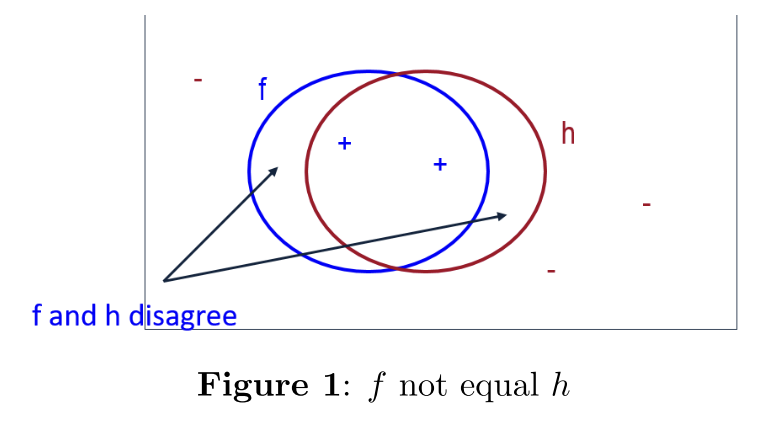
\includegraphics[width=0.5\textwidth]{eg1.png} % 插入图片,设置图片宽度为0.5倍文本宽度
\end{figure*}
In this example, $x_1$ in all positive training instances. Therefore, it is very likely that it will be active in future positive examples. If not, it is active in only a small percentage of examples, so the error should be small.

\section{Conjunction}
\subsection{Error Bounds}
$Claim: \ Error(h) \leq \sum_{z\in h} p(z).$
\begin{itemize}
    \item $p(z)$: the probability that a D-sampled example is positive and $z$ is false in it (like $x_1$ in eg1).(\textcolor{lightBlue}{type1-error? I in FDP?})
\end{itemize}
$Claim $: It there are no bad literals, then $Error(h) < \epsilon.$
\subsection{Example \textbf{\textcolor{lightBlue}{(just examble... to be deleted)}}}
\begin{example}
    The core idea of PAC-learnability is easy to understand, and we’ll start with a simple example to explain it. 
    Imagine a game between two players. Player 1 generates numbers $x$
    at random in some fixed way, and in Player 1’s mind he has an interval $[a, b]$. 
    Whenever Player 1 gives out an $x$, he must also say whether it’s in the interval 
    (that is, whether $a \leq x \leq b$). Let’s say that Player 1 gives reports a 1 if $x$ is in the interval, and a 0 otherwise. 
    We’ll call this number the label of $z$, and call the pair of ($x$, label) a sample, or an example. 
    We recognize that the zero and one correspond to “yes” and “no” answers to some question 
    (Is this email spam? Does the user click on my ad? etc.), and so sometimes the labels are instead $\pm 1$, and referred to as “positive” or “negative” examples. 
    We’ll use the positive/negative terminology here, so positive is a 1 and negative is a 0.
    \\Player 2 (we’re on her side) sees a bunch of samples and her goal is to determine $a$ and $b$. 
    Of course Player 2 can’t guess the interval exactly if the endpoints are real numbers, because Player 1 only gives out finitely many samples. 
    But whatever interval Player 2 does guess at the end can be tested against Player 1’s number-producing scheme. 
    That is, we can compute the probability that Player 2’s interval will give an incorrect label if Player 1 were to continue giving out numbers indefinitely. 
    If this error is small (taking into account how many samples were given), then Player 2 has “learned” the interval. 
    And if Player 2 plays this game over and over and usually wins (no matter what strategy or interval Player 1 decides to use!), then we say this problem is PAC-learnable.
\end{example}
PAC stands for Probably Approximately Correct, and our number guessing game makes it clear what this means. Approximately correct means the interval is close enough to the true interval that the error will be small on new samples, 
and Probably means that if we play the game over and over we’ll usually be able to get a good approximation. 
That is, we’ll find an approximately good interval with high probability.

Indeed, one might already have a good algorithm in mind to learn intervals. Simply take the largest and smallest positive examples and use those as the endpoints of your interval. 
It’s not hard to see why this works, but if we want to prove it (or anything) is PAC-learnable, then we need to solidify these ideas with mathematical definitions.


\section{Formulating Prediction Theory}
\begin{itemize}
    \item This notion relies on the \textcolor{lightBlue}{Consistent Distribution Assumption}: there is one probability distribution $D$ that governs both training and testing examples.
\end{itemize}
(what's the meaning of 'governs'? like 'dominate'? how does it been defined?)
\subsection{PAC introduction}
Definitions and Notation:
\begin{itemize}
    \item $X$: set of all possible instances or examples, e.g., 
    the set of all men and women characterized by their height and weight.
    \item $c: X \rightarrow \{0, 1\}$: the target concept to learn; can be identified with its support $\{x \in X: c(X)=1\}$.
    \item $C$: concept class, a set of target concepts $c$.
    \item $D$: target distribution, a fixed probability distribution over $X$. Training and test examples are drawn according to $D$.
    \item $H$: training sample.
    \item $S$: set of concept hypotheses, e.g., the set of all linear classifiers. 
\end{itemize}
The learning algorithm receives sample and selects a hypothesis $h_S$ from $H$ approximating.
\\\textit{Any (efficient) algorithm that returns hypotheses that are PAC is called a PAC-learning algorithm. 
(Formal definition to be introduced later)} \textit{\textcolor{lightBlue}{? Explainaiton in slides-W14 Wu Peiyuan}}
\begin{definition}
    True error or generalization error of $h$ with respect to the target concept $c$ and distribution $D$:
    \begin{equation*}
        Error(h)=\operatorname{Pr}_{x \sim D}[h(x) \neq c(x)]=\underset{x \sim D}{\mathrm{E}}\left[1_{h(x) \neq c(x)}\right] .
    \end{equation*}    
\end{definition}
\begin{definition}
    Empirical error: average error of $ h $ on the training sample $ S $ drawn according to distribution $ D $,
    \begin{equation*}
        \widehat{Error}_{S}(h)=\operatorname{Pr}_{x \sim \widehat{D}}[h(x) \neq c(x)]=\operatorname{E}_{x \sim \widehat{D}}\left[1_{h(x) \neq c(x)}\right]=\frac{1}{m} \sum_{i=1}^{m} 1_{h\left(x_{i}\right) \neq c\left(x_{i}\right)} .
    \end{equation*}
\end{definition}
Note: $ Error(h)=\underset{S \sim D^{m}}{\mathrm{E}}\left[\widehat{R}_{S}(h)\right]$.
\\ \textbf{A few comments on notation.} $\epsilon$ is called the accuracy parameter, and we call h “$\epsilon $-good”
if $Error(h) \leq \epsilon $, where $Error(h)$ is called the true error or the generalization error. $\delta$ is
the confidence parameter.
\\ \textit{\textcolor{lightBlue}{The
name “Probably Approximately Correct” comes from the fact that we want a hypothesis
that is approximately correct ($\epsilon $-good) with high probability (namely $1- \delta$).}}

\subsection{PAC Learnability}
Consider a concept class $C$ defined over an instance space $X$, and a learner $L$
using a hypothesis space $H$. Denote as $Error(h)$ as $\mathcal{R}(h)$. 
\begin{definition}
    $C$ is PAC learnable by $L$ using $H$ if:
    $\forall f \in C$, $\forall D$ over $X$, and fixed $0 < \epsilon, \delta < 1$, L – given a collection of $m$ examples sampled independently according to D – produces with probability at 
    least $1 - \delta$ a hypothesis $h \in H$ with error at most $\epsilon$ where $m$ is polynomial in $\frac{1}{\epsilon}, \frac{1}{\delta}$ and $|H|$.
    \begin{equation*}
        \operatorname{Pr}_{S \sim D^m}[\mathcal{R}(h(S)) \leq \epsilon] \geq 1- \delta,
    \end{equation*}
    where $h(S) \in H$ is the hypothesis learned by $\mathbb{A}$ from sample $S$. We say $\mathbb{A}$ is a PAC-learning algorithm for $C$.
\end{definition}
Another definition of PAC learning:
\begin{definition}
    Concept class $C$ is PAC-learnable if there exists a learning algorithm such that:
    \begin{itemize}
        \item for all $c \in C, \epsilon > 0, \delta > 0$ and all distributions $D$, $\underset{S \sim D^{m}}{\operatorname{Pr}}[R_{S}(h) \leq \epsilon] \geq 1-\delta$
        \item for samples $S$ of size $m = poly(1/\epsilon, 1/\delta)$ for a fixed polynomial.
    \end{itemize}
\end{definition}

\begin{theorem}
    Sample complexity for finite hypothesis sets - consistent case: 
    Let $H$ be a finite set of binary classifiers on $\mathrm{X}$. Let $A$ be an algorithm 
such that for any target concept $c \in H$ and i.i.d. sample $S$ of size $m$ returns a 
consistent hypothesis $\mathbb{A}(S) \in H$ such that $\widehat{\mathcal{R}}_S(\mathbb{A}(S))=0$. Then 
\begin{equation*}
    \operatorname{Pr}_{x \sim \widehat{D}}[\mathcal{R}(\mathbb{A}(S)) \leq \epsilon] \geq 1- |H|e^{-m\epsilon}
\end{equation*}
\end{theorem}


\newpage
\bibliographystyle{plain}
\bibliography{ref}
\end{document}